\documentclass[colorlinks=true,pdfstartview=FitV,linkcolor=blue,
            citecolor=red,urlcolor=magenta]{ligodoc}

\usepackage{graphicx}
\usepackage{amssymb}
\usepackage{amsmath}
\usepackage{longtable}
\usepackage{rotating}
\usepackage[usenames,dvipsnames]{color}
\usepackage{fancyhdr}
\usepackage{subfigure}
\usepackage{hyperref}
% \usepackage{minted}
\usepackage{appendix}
\usepackage{tikz}
\usetikzlibrary{shapes,arrows,fit}
\ligodccnumber{T}{19}{00287}{}{v1}% \ligodistribution{AIC, ISC}


\title{Data Clustering Techniques for the Correlation of Environmental Noise to Signals in LIGO Detectors}

\author{Jacob Bernhardt, Anamaria Effler, Rana Adhikari}

\begin{document}

\section{Introduction}
The LIGO project uses laser interferometry to measure gravitational waves (GWs).
LIGO interferometers transduce their relative arm length differences caused by GWs to a signal composed of optical power, known as DARM.
Due to the amplitude scales of astrophysical GWs, The LIGO detectors have to operate at a very high sensitivity; the spectral density of a measurable length difference is as low as $2\times 10^{-20}~\mathrm{m}/\sqrt{\mathrm{Hz}}$ at 100 Hz.
The design of earthbound LIGO is thus heavily focused on the filtering and isolation of environmental noise.

To help identify and characterize environment-based noise, the LIGO detector has a Physical Environment Monitoring (PEM) system, a diverse array of environmental sensors positioned all over the facility\cite{aepaper}.
This is used for a multitude of purposes, including the data quality report (DQR) used for time segment vetoing, based on direct coherence of PEM channels to DARM.
Supplementing coincidence analysis between the two detectors, DQR prevents GW-like noise transients from being falsely categorized as events.
Thus, detector livetime can be increased by figuring out how to decouple environmental noise from DARM.
Directly coupling noise, found by basic coherence, has been already addressed, but the complexity of the detector causes many noise sources to up- or down-convert.
These require some more careful statistical correlation to identify, and are sometimes not well understood.
\begin{figure}
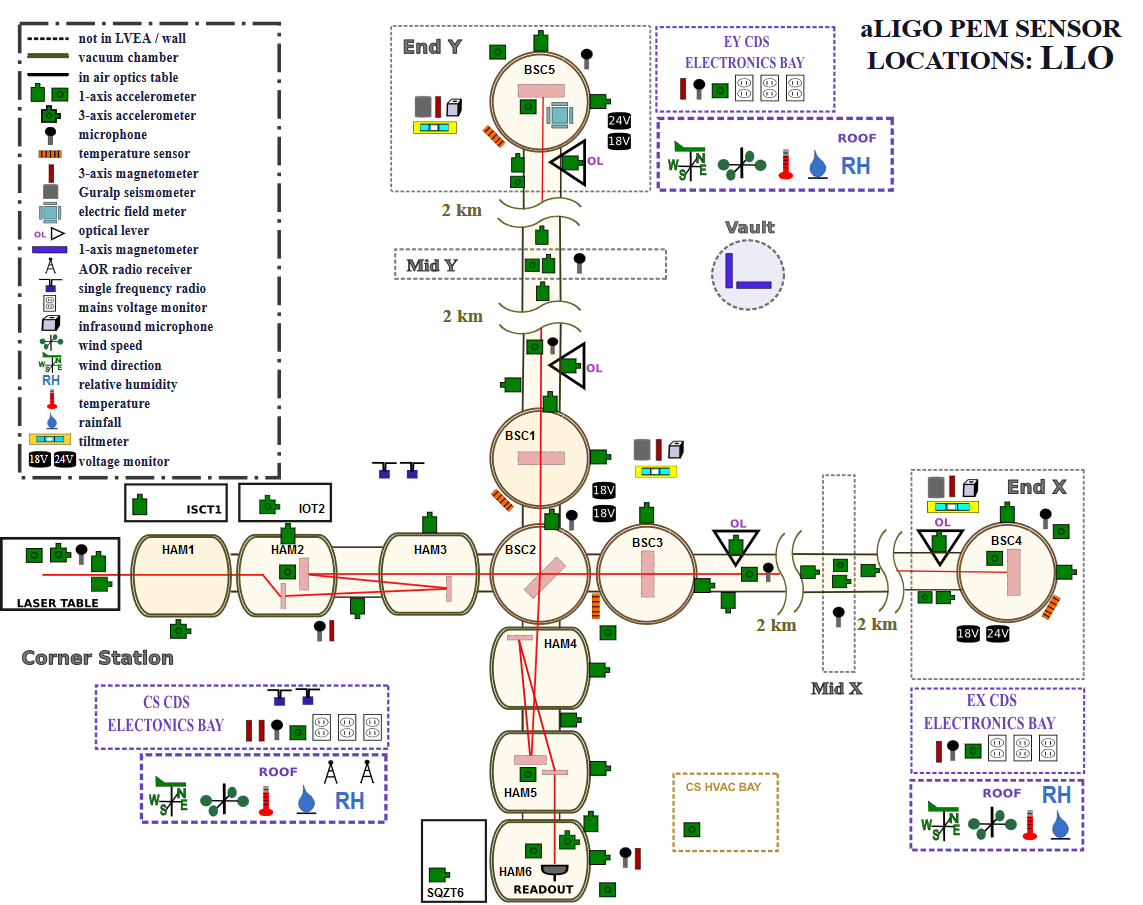
\includegraphics[width=\textwidth]{assets/llopem.png}
\caption{Schematic PEM map at the LIGO Livingston Observatory (L1). Shaded areas are in vacuum.}
\end{figure}
\begin{figure}
  \begin{minipage}[c]{0.67\textwidth}
  \begin{tabular}{c}
  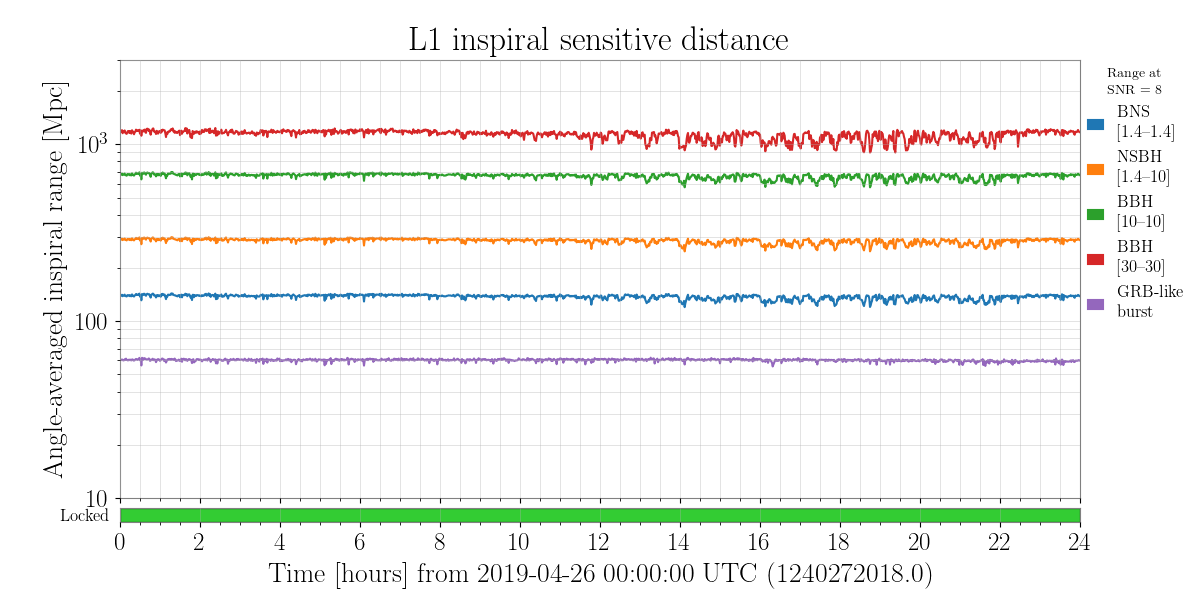
\includegraphics[width=\textwidth]{assets/L1-LOCKED_216737_RANGE-1240272018-86400.png}   \\  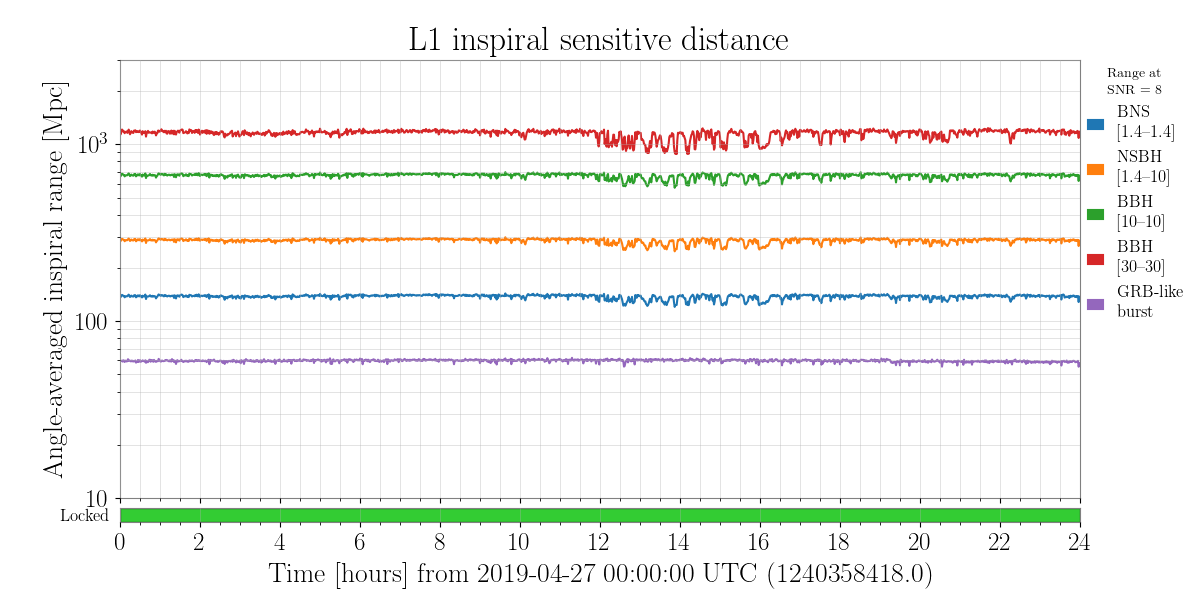
\includegraphics[width=\textwidth]{assets/L1-LOCKED_216737_RANGE-1240358418-86400.png}
  \end{tabular}
  \end{minipage}\hfill
  \begin{minipage}[t]{0.3\textwidth}
    \caption{Detector range at L1 seems to consistently reduce during the day ($\sim$6am-5pm CST). For large BBH in these plots, the reduction is about 300 Mpc. The source of this has been pinpointed to the Y end station, but the mechanism isn't fully clear.}
  \end{minipage}
\end{figure}

Separating noise sources out of a signal can be considered a clustering problem in a space covering different frequency bands in which noise appears.
A previous LIGO SURF student has evaluated several data clustering algorithms with respect to their ability to properly sort out frequency elements of seismometer signals caused by specific earthquake events\cite{roxana}.
Both the $k$-means algorithm, which aims to make clusters with low standard deviation, and the DBSCAN algorithm, which minimizes overall inter-point distance in clusters, were evaluated using multiple methods, including the Calinsky-Harabaz  index and direct comparison to earthquake times via time labeling of points, ultimately showing poor earthquake identification.
A long short-term memory (LSTM) recurrent neural network (RNN) seemed to work much better, but due to small input sample size, this solution may have been be plagued by over-fitting.
Thus, it is imperative that a more robust frequency clustering mechanism be designed for the PEM system.

\section{Objectives}
% What do you aim to accomplish in your project? What will you measure, and under what conditions; or, what will you calculate, model, or simulate; or what will you design, and what are the requirements; or what will you build or test? What is your starting point? What are your initial assumptions or conditions? What will be the result or product of a successful outcome for your project? What are the criteria for project completion or for success? (In other words, how will you know when you have accomplished what you set out to do?)
\begin{itemize}
\item
As a primary goal, \textbf{algorithms or clustering approaches which correctly identify known noise events need to be found}.
As every algorithm has inbuilt assumptions about the dataset it is applied to, the results of an algorithm performance test on labeled data will yield information about the structure of the data.
The general temporal non-stationarity of the DARM noise will need to be accounted for by varying testing time windows.
\item
The secondary goal is to \textbf{create a clustering approach to discover previously unknown noise correlations and possibly sources}.
This is where the ``detector characterization tool'' that this project aims to advance will be functional---revealing new noise coupling pathways will help identify ways to improve the detector sensitivity.
\end{itemize}

\section{Approach}
% Specifically, how will you reach your objective or produce your desired final product? What are the principal steps or milestones along the path? How long will each take? What steps promise to be the most difficult, and how will you overcome the difficulties? What equipment or other resources will you need? Which of these are inherited, and which will you have to make or procure? With what other people or groups will you be collaborating? Will completion of your project depend on results from other people in related projects? (That question may be especially pertinent for team projects.)

Initially, a program will be written to take the spectral power of any PEM channel, in the form of band-limited RMS (BLRMS), likely using established methods like looping through a smoothed spectogram of the channel\cite{vajente}.

To reach the first objective, a modular \texttt{python} testing suite will be written to probe the structure of the multidimensional frequency-domain sensor data.
This will strategically implement \texttt{scikit-learn} clustering algorithms and classifiers with different optimal regimes of function or working assumptions and evaluate them using point labeling. 
This will require, additionally to researching clustering or unsupervised classification algorithms, thinking of as many variables which may affect the data structure (such as looking at different time windows) and intelligently testing them. 
Optimizations will need to be considered so that run times are reasonable.

The program tackling the second objective will use working clustering approaches identified in the first objective to find new noise correlations.
In the event that no individual algorithm or technique outperforms the rest for all types of sensory data, the final program will use the modular programming environment created for the testing suite to match techniques to the regimes that they work in.
The structure of the input data as determined by the first objective, including the dimensionality probed by the extra variables, may lend itself to additional algorithms that can be used to combine the target regimes.
To this end, extra algorithm research will be conducted with specific consideration of the solved structure.

%%% Local Variables:
%%% mode: latex
%%% TeX-master: "../proposal"
%%% End:


\section{$k$-Means Clustering with Histories}
The $k$-means algorithm was used to cluster the two hours of minute-trend data preceding each point in time.
The coordinates of a clustered point were as follows:
\begin{equation}
  \begin{array}{c}
    \{s_0(t_0),s_0(t_{-1}),s_0(t_{-2}),\cdots,s_0(t_{-n}),\\
    s_1(t_0),s_1(t_{-1}),s_1(t_{-2}),\cdots,s_1(t_{-n}),\\
    s_2(t_0),s_2(t_{-1}),s_2(t_{-2}),\cdots,s_2(t_{-n}),\\
    \cdots,\\
    s_m(t_0),s_m(t_{-1}),s_m(t_{-2}),\cdots,s_m(t_{-n})\}
  \end{array}
\end{equation}
with $s_j(t)$ the value of a clustered channel $j$ at time $t$ in its own units, e.g. a seismometer velocity at time $t$.
Each dimension could be thought of as ``value of specific channel a specific number of minutes ago'', allowing trends over time to be matched together in a phase-agnostic way.
This yields a cluster space of dimensionality (\# of channels) $\times$ (\# of minutes of history).

Notably, the clustering endeavored by \cite{roxana} lacked this history feature, using a clustering space of dimensionality (\# of channels) $\times$ (1).
Instead of just finding times when the channels are similar in value, the history clustering is sensitive to the shape of clustered features.

\begin{figure}[h]
  \tikzstyle{block} = [rectangle, draw, text width=6em, text centered, rounded corners, minimum height=4em]
  \begin{tikzpicture}[node distance = 9em, auto]
    \node [block] (dl) {get minute-trend data from NDS};
    \node [block, right of=dl] (input) {create input matrix};
    \node [block, right of=input] (compute) {compute $k$-means clusters};
    \node [block, right of=compute] (save) {save labels};
    \draw [->] (dl) -- (input);
    \draw [->] (input) -- (compute);
    \draw [->] (compute) -- (save);
  \end{tikzpicture}
  \caption{Clustering script flowchart.}
\end{figure}

\subsection{Sanity Checking with Seismometers}
For a total clustering duration of 30 days, using the seismometers attached to ETMY, ETMX, and ITMY, in minute-trend half-order-of-magnitude BLRMS bands from 30 mHz to 30 Hz, the following known noise events were easily identified using a ``2-hour history'' $k$-means method:
\begin{itemize}
\item earthquakes ($0.01\to0.1$ Hz)
\item microseisms ($0.1\to1$ Hz)
\item anthropogenic noise ($1\to10$ Hz)
\end{itemize}

Some differentiation between subcategories of events in the same frequency band but of different timescales (e.g. earthquakes vs. wind; train vs. noise from cars) was lacking.

The length of the history was initially thought to have an effect on the timescales of identifiable events; experimentation (namely, trying 30-minute and 6-hour histories on the same data) showed that this is not really true.

The next idea was that there were too many different types of features in too large a space for events with a small number of points, like the trains, to be separated out.
The test was re-run with only anthropogenic seismic BLRMS bands at the end stations, which yielded very clear distinction between the anthropogenic noise types.

\section{Clustering with DARM BLRMS}
Now that the clustering scheme is verified using known states of noise, it can be used to find new relationships between PEM channels and DARM noise.

\subsection{Seismometers}

\subsection{Accelerometers}

\subsection{Microphones}

\section{Developed Code Tools: Optimizations and Considerations}
Many times, scientists are inclined to launch REPLs and quickly do their simple calculations imperatively.
But time and RAM are not infinite, and with a high-output experiment like LIGO the usual kinds of scripts and operations do not suffice.
Given that much of the summer was spent figuring out how to write robust code that can handle large-scale data, rather than actually doing science, it is worth mentioning the way this was accomplished.

\subsection{Streaming}
One data-wrangling strategy is by programming with a ``streaming'' rather than ``batch'' mentality.
Many of the gravitational wave search pipelines have the ability to keep up with new LIGO data as it is collected, doing their batch-style work in short chunks, or strides, as the data comes along.
This keeps the execution footprint of the program managable, while allowing it to operate on an unending amount of data.

The Python package \texttt{GWpy}, used in this project, is the modern equivalent to LIGO's Algorithms Library, a set of common routines designed for LIGO data.
Strangely, appending to HDF5 savefiles, a streaming requisite, is not possible in \texttt{GWpy} without some lower-level calculations using the \texttt{libhdf5} wrapper directly and likely unintented \texttt{GWpy} keyword-argument usage.

Two helper functions, \texttt{write\_to\_disk} and \texttt{data\_exists}, were defined in \texttt{util.py} for the purpose of apppending a time series to an existing file and quickly checking the length of saved data without reading it.

A Python module was written to implement the ``streaming'' idea for any given batch operation.
One such task is the computation of BLRMS for channels that don't provide it in DMT frames.
The BLRMS-generating function is an implementation of a general \texttt{PostProcessor} interface, a \texttt{python3.7} dataclass which is fed INI options upon construction (see Figure~\ref{fig:pp}).
\begin{figure}[h]
  \tikzstyle{block} = [rectangle, draw, text width=6em, text centered, rounded corners, minimum height=4em]
  \tikzstyle{section} =[rectangle, draw, inner sep=1.125em, dashed]
  \begin{tikzpicture}[node distance = 9em, auto]
    \node [block] (dl) {get data from NDS or savefiles};
    \node [block, below of=dl] (strides) {compute strides};
    \node [block, right of=strides] (next) {get next stride};
    \node [block, below of=next] (stride) {extract stride};
    \node [block, right of=stride] (compute) {compute spectogram};
    \node [block, right of=compute] (add) {add power within requested bands};
    \node [block, right of=add] (save) {stitch stride into .hdf5 file};
    \node [block, below of=add] (shape) {read .hdf5 dataset shape};
    \node [block, below of=save] (offset) {compute offset};
    \node [section, label=below:BLRMS \texttt{PostProcessor}, fit=(add) (compute)] (blrms) {};
    \node [block, above of=blrms, node distance = 18em, dashed] (load) {load INI section};
    \draw [->] (dl) -- (strides);
    \draw [->] (strides) -- (next);
    \draw [->] (next) -- (stride);
    \draw [->] (stride) -- (compute);
    \draw [->] (compute) -- (add);
    \draw [->] (add) -- (save);
    \draw [->] (stride) |- (shape);
    \draw [->] (shape) -- (offset);
    \draw [->] (offset) -- (save);
    \draw [->] (save) |- (next);
    \draw [->, dashed] (load) -- (blrms);
    \draw [->, dashed] (load) -- (dl);
  \end{tikzpicture}
  \caption{States of the ``streaming post-processor'' script.}\label{fig:pp}
\end{figure}

Any data processing function which maps an input channel to an output channel and has tons of configuration parameters can take advantage of the module by implementing the \texttt{PostProcessor} interface.
Indeed, converting saved channels to minute-trend and caching NDS downloads in the same format were easy last-minute tasks with this generic structure in place.

\subsection{Evaluation of Clusters}
The clustering script itself was fairly straightforward, using the high abstraction provided by \texttt{scikit-learn}.
However, some thought was put into extracting meaning from the clusters.

A script was created to make power spectra for the clustered data representative of each cluster.
This is done by taking the median of the power spectra for many time intervals clustered together.
\begin{figure}[h]
  \tikzstyle{block} = [rectangle, draw, text width=6em, text centered, rounded corners, minimum height=4em]
  \tikzstyle{section} =[rectangle, draw, inner sep=1.125em, rounded corners, ->]
  \begin{tikzpicture}[node distance = 9em, auto]
    \node [block] (labels) {read labels};
    \node [block, left of=labels] (filter) {locate base cluster};
    \node [block, left of=filter] (segments) {locate non-base cluster segments};
    \node [block, left of=segments] (dl) {download full-rate minutes in segments};
    \node [block, below of=segments] (psd) {take  psd for each minute in the cluster};
    \node [block, right of=psd] (median) {plot median};
    \node [section, label=above:for each cluster, fit=(psd) (median)] (cluster) {};
    \draw [->] (labels) -- (filter);
    \draw [->] (filter) -- (segments);
    \draw [->] (segments) -- (dl);
    \draw [->] (dl) |- (cluster);
    \draw [->] (psd) -- (median);
  \end{tikzpicture}
  \caption{Roughly the states of the ``representative spectra'' script. The most complicated overlooked detail in this figure is the caching of downloads. The stream writing functions used in the BLRMS-generation script have been moved and are now included from a more general location.}
\end{figure}

Taking the spectra of the clusters provides a signature for each cluster that can be programmatically validated, allowing new states to be detected without re-clustering, and also a way to easily identify frequency conversion that is happening during coupling.
The script can extract other attributes that are helpful for chasing down the source and eliminating it, like the periodicity or dominating channels.
\begin{figure}
  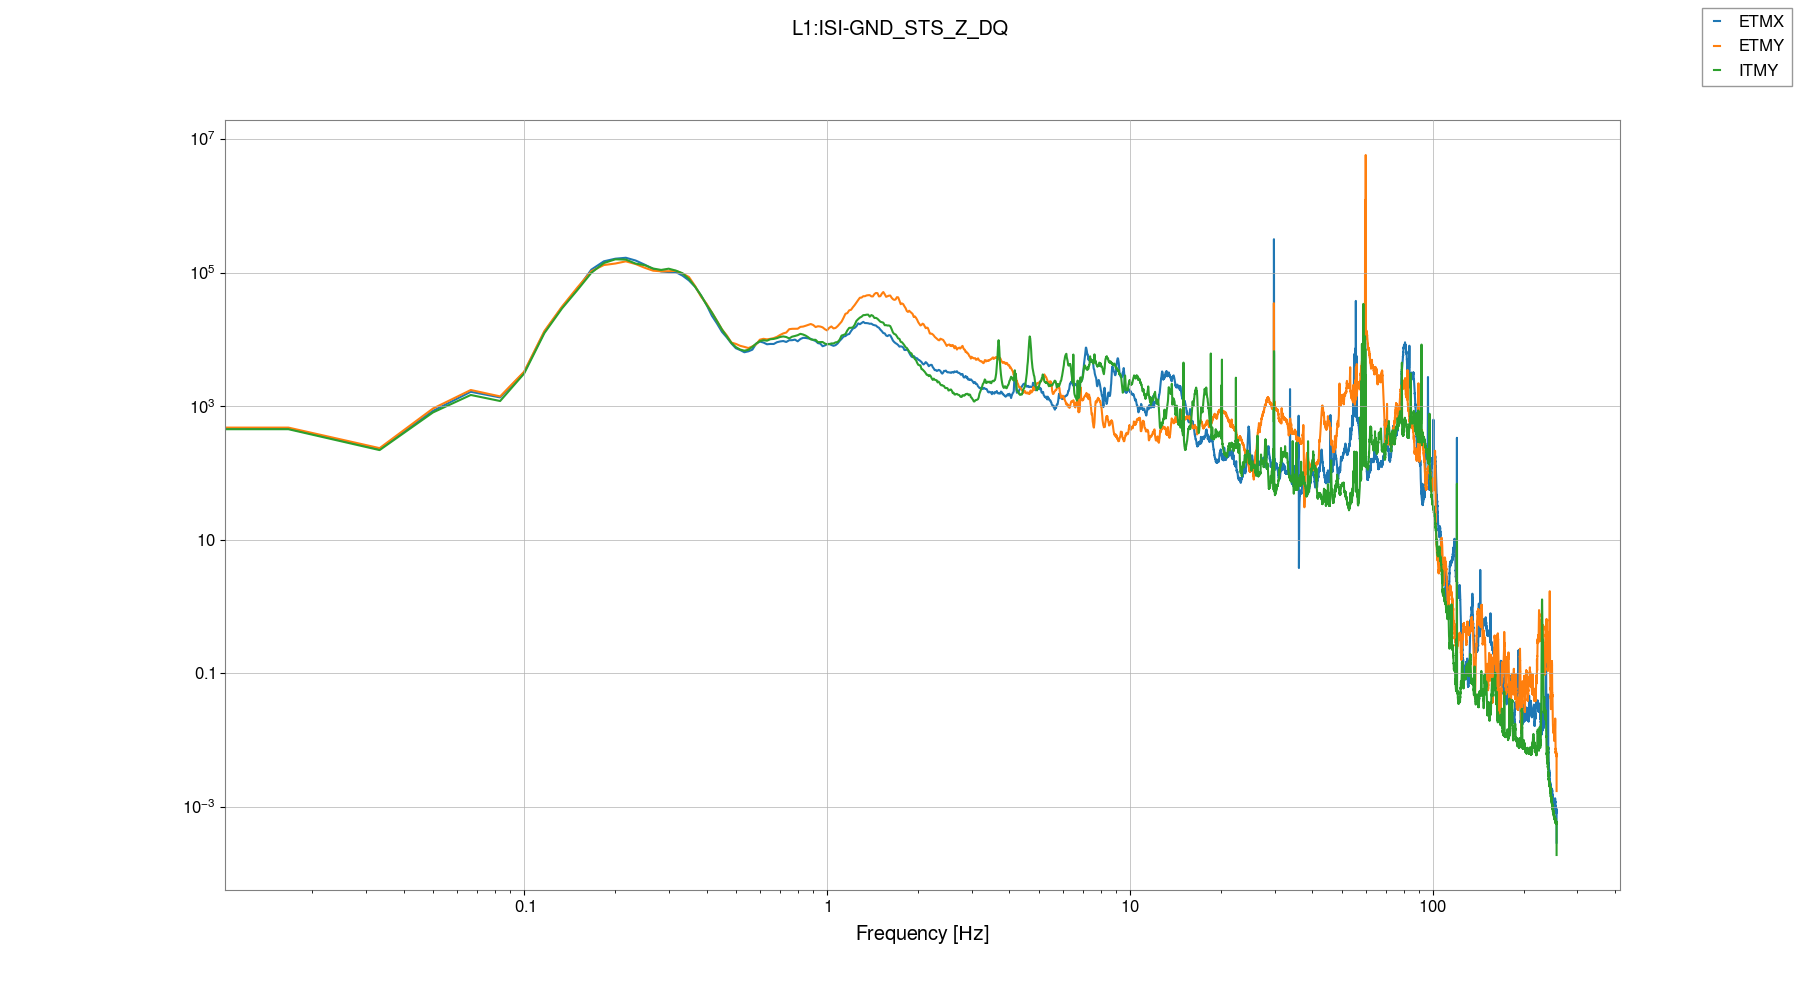
\includegraphics[width=\textwidth]{assets/report2/0-L1:ISI-GND_STS_Z_DQ.png}
  \caption{The representative spectrum of a cluster corresponding to train-dominated times. Notice that between 1 and 10 Hz, the seismic motion at ETMY (orange) is greater than at the other VEAs by a factor of about 10.}
\end{figure}

In addition, the script can produce a table that shows which frequency bands are significant in each channel during clustered times.
``Significance'' is established by determining if the average BLRMS value at clustered times is not close to the BLRMS value of ``unclustered'' times, or times in the base cluster representing ``everything else''.


\appendix
\appendixpage
\section{Resampling}
Downloading and saving full-rate data takes an exorbitant amount of disk space, especially when only a portion of the frequency content is going to be used.
This calls for a decimation procedure to be applied to raw downloads before they are saved.

At CIT, Rana mentioned that the default low-pass filtering options in scipy's resampling function produce significant aliasing noise ($>1$\%) when downsampling by a large factor.
According to a test\footnote{see \url{https://git.ligo.org/NoiseCancellation/GWcleaning/issues/2}} done by Eric Quintero, this issue can be remedied without sacrificing runtime by using (1) a number of FIR taps proportional to the downsampling factor, rather than the default fixed value, and (2) a non-default window (\texttt{blackmanharris}).

% FIXME: figure of window comparison

For a full-rate time series \texttt{raw: gwpy.timeseries.TimeSeries}, the fastest and best procedure for resampling to \texttt{rate: int [Hz]} would be something like
% \begin{minted}[style=colorful]{python}
\begin{verbatim}
raw.resample(n=20*raw.sample_rate.value/rate, window='blackmanharris', rate=rate)
\end{verbatim}
% \end{minted}

\section{Evaluation of Non-$k$-means Clustering Algorithms}
A test\footnote{\url{https://scikit-learn.org/stable/auto_examples/cluster/plot_cluster_comparison.html}} which swaps out the $k$-means algorithm for others implemented in \texttt{sklearn} was executed to probe the geometry of the clusters.
From a first glance, the Spectral Clustering and Gaussian Mixture algorithms seemed to generalize better than $k$-means over different feature timescales.
However, algorithm upgrades are helpful only after tools for full cluster analysis are in place, and due to time limitations they were not revisited.

\begin{thebibliography}{2}
\bibitem{aepaper} A. Effler, R. M. S. Schofield, V. V. Frolov, G. Gonz{\'{a}}lez, K. Kawabe, J. R. Smith, J. Birch, and R. McCarthy, Classical and Quantum Gravity \textbf{32}, 035017 (2015).
\bibitem{roxana} LIGO Document T1700198-v1
\bibitem{vajente} aLIGO LLO Logbook entry 45374 by Gabriele Vajente
\end{thebibliography}



\end{document}
